\documentclass[11pt]{scrartcl}

\title{Anforderungsspezifikation}
\author{Silvan Adrian \\ Fabian Binna \\ Pascal Kistler}
\date{\today{}}

\usepackage[ngerman]{babel}
\usepackage[automark]{scrpage2}
\usepackage{hyperref}
\usepackage{color}
\usepackage[normalem]{ulem}
\usepackage{scrpage2}
\usepackage{graphicx}
\usepackage{tabularx}
\usepackage{sidecap}
\graphicspath{ {./images/} }
\pagestyle{scrheadings}
\usepackage{wrapfig}
\usepackage{longtable, tabu}

\clearscrheadfoot
\ihead{
\includegraphics[scale=0.4]{jbomberman}}
\ohead{Projekt: JBomberman}
\ifoot{Anforderungsspezifikation}
\cfoot{Version: 1.00}
\ofoot{Datum: \today{}}
\setheadsepline{0.5pt}
\setfootsepline{0.5pt}

\usepackage{ucs}
\usepackage[utf8]{inputenc}
\usepackage[T1]{fontenc}


\begin{document}
\def\arraystretch{1.5}
\begin{titlepage}
\begin{center}
\vspace{10em}

\includegraphics[scale=2]{jbomberman}
\vspace{10em}
\end{center}
\begin{center}
\huge {Projekt: JBomberman} \\
\huge {Anforderungsspezifikation}
\end{center}
\begin{center}
\vspace{10em}
\LARGE {Pascal Kistler} \\
\LARGE {Silvan Adrian} \\
\LARGE {Fabian Binna}
\end{center}

\end{titlepage}

\newpage
\section{Änderungshistorie}
\label{sec:Änderungen}

\begin{tabularx}{\linewidth}{l l l l}
\textbf{Datum} & \textbf{Version} & \textbf{Änderung}  & \textbf{Autor} \\
\hline
\textbf{09.03.15} & 1.00 & Erstellung des Dokuments & Gruppe \\
\textbf{12.03.15} & 1.01 & detailliertes Spielprinzip schreiben & Silvan Adrian \\
\textbf{13.03.15} & 1.02 & Spielregeln im detail & Silvan Adrian \\
\end{tabularx}

\newpage
\tableofcontents
\newpage
\section{Einführung}
\label{sec:Einführung}

\subsection{Gültigkeit}
\label{sec:Gültigkeit}
Dieses Dokument ist während des ganzen Projekts gültig und wird laufend aktualisiert.
\subsection{Referenzen}
\label{sec:Referenzen}
siehe letzte Seite Literatur

\subsection{Übersicht}
\label{sec:Übersicht}

\section{Allgemein Beschreibung}
\label{sec:Allgemeine Beschreibung}

\subsection{Produkt Perspektive}
\label{sec:Produkt Perspektive}

\subsection{Produkt Funktion}
\label{sec:Produkt Funktion}

\subsection{Benutzer Chrakteristik}
\label{sec:Benutzer Chrakteristik}

\subsection{Einschränkungen}
\label{sec:Einschränkungen}

\subsection{Annahmen}
\label{sec:Annahmen}

\subsection{Abhängigkeit}
\label{sec:Abhängigkeit}
\newpage
\section{Detailiertes Spielprinzip}
\label{sec:Detailiertes Spielprinzip}
\subsection{Kurzbeschreibung}
\label{Kurzbeschreibung}
In der klassischen Variante besteht das Spielfeld aus einer Anordnung 
von zerstörbaren und unzerstörbaren Wänden. 
Durch das Legen von Bomben können somit immer mehr 
Bereiche des Spielfelds erschlossen werden. Hinter einigen 
Wänden verstecken sich Bonusgegenstände.\cite{Bomberman Spielprinzip}

\subsection{Spielregeln}
\label{sec:Spielregeln}

\subsubsection{Spielewinn}
\label{sec:Spielgewinn}
Ein Spieler hat gewonnen, wenn alle anderen Bombermans besigt sind und er der letzte bestehende Spieler auf dem Spielfeld ist.
Der Gewinner bekommt einen Punkt für die gewonnene Runde und wird im angerechnet angezigt in der Statusanzeige.

\subsubsection{Spielabbruch}
\label{sec:Spielabbruch}
Zu einem Spielabbruch kommt es, wenn es zu wenige Mitspieler gibt (mindestens 2 Spieler müssen verbunden sein).
Dies kann passieren, falls ein Verbindungsunterbruch passieren sollte.

\subsubsection{Timer läuft ab}
\label{sec:Timer läuft ab}
Falls innerhalb der festgelegten Zeit kein Bomberman alle anderen Mitspieler besiegt wird das Spielfeld verkleinert.
Die Bomberman, die sich dabei auf einem Block befindet der \grqq{}verschwindet\grqq{} wird aus dem Spiel geworfen.
Der Bomberman, der übrig bleibt wird dabei der Gewinner der Spielrunde.

\subsubsection{Bombe}
\label{sec:Bombe}
Sobald eine Bombe platziert ist wird desen \grqq{}Zeit bis zur Explosion gestartet\grqq{}.
Sobald ein Bombe explodiert wird alles was sich im Radius der Bombe befindet und zerstörbar ist zerstört.
Der Radius der Bombeexplosion kann varieren, da Powerups für das erhöhen des Bombenradius bestehen.
\subsubsection{Zerstörbare Wand}
\label{sec:Zerstörbare Wand}
Wenn eine zerstörbare Wand zerstört wird verschwindet diese.
Manche zerstörbaren Gegenstände beherbergen Powerups für die Bomberman, welche nach dem zerstören der Wand aufgedeckt werden.
Solange die Wand aber nicht zerstört ist kann auch kein Bomberman diese durchqueren.

\subsubsection{Unzerstörbare Wand}
\label{sec:Unzerstörbare Wand}
Unzerstörbare Wände können nicht durch Bomben zerstört werden, noch von Bombermans durchquert werden.

\subsubsection{Bomberman}
\label{sec:Bomberman}
Der Bomberman wird über die Tastatur gesteuert, dabei gibt es 4 Tasten für die Fortbewegung und 1 Zusätzliche Taste für das legen der Bombe.
Ein Bomberman kann sich \grqq{}upgraden\grqq{} wenn er Powerups aufnimmt.

\subsection{Spielelemente}
\label{sec:Spielelemente}
\subsubsection{Statusanzeige}
\label{sec:Statusanzeige}
In der Statusanzeige wird für jeden einzelnen Bomberman (1-4 Spieler) die Anzahl 
Gewinne und ein Timer der runterzählt angezeigt.
\subsubsection{Spielfeld}
\label{sec:Spielfeld}
Das Spielfeld wird sich auf eine Grösse von ca. 13 Blöcken x 13 Blöcken 
erstrecken.
Die Wände sind dabei unzerstörbar, damit die bis zu 4 Bombermans das Spielfeld 
nicht verlassen können.
Jeder Ecken im Spielfeld ist für einen Bomberman festgelegt, bei weniger als 4 
Spielern bleiben die übrigen Ecken einfach leer.

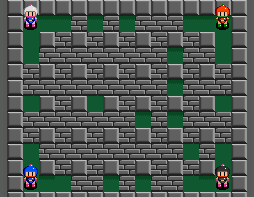
\includegraphics[scale=1.5]{bombermanmap} 

\cite{Bomberman Spielfeld}
\newpage
\subsection{Wände}
\label{sec:Wände}
\subsubsection{Unzerstörbar}
\label{sec:Unzerstörbar}
\begin{table}[!h]
\begin{tabularx}{\linewidth}{l X }
     
      \raisebox{-.8\totalheight}{ 
\includegraphics[scale=.8]{solidblock}}
      & Die unzerstörbaren Wände können von keiner Bombe zerstört noch von einem 
Bomberman durchlaufen werden.
\end{tabularx}
\end{table}


\subsubsection{Zerstörbar}
\label{sec:Zerstörbar}

\begin{table}[!h]
  \begin{tabularx}{\textwidth}{l X }
    
    
       \raisebox{-.8\totalheight}{
\includegraphics[scale=0.8]{explodableblock}} & Die zerstörbaren Wände können von 
    einer Bombe zerstört werden, bevor sie zerstört sind kann ein Bomberman 
    diese nicht durchlaufen.
  \end{tabularx}
\end{table}
\subsection{Bomberman}
\label{sec:Bomberman}
\begin{table}[!h]
\begin{tabularx}{\textwidth}{l X}
\raisebox{-.8\totalheight}{
\includegraphics[scale=0.6]{bomberman}}
  & Der Bomberman ist der steuerbare Charakter im Bomberman Spiel, dabei kann er 
sich in alle Himmelsrichtungen bewegen.
Es sei denn ein Hindernis ist im Weg, dann kann er sich nicht weiter bewegen.
\end{tabularx}
  
\end{table}



\subsection{Bombe}
\label{sec:Bombe}
\begin{table}[!h]
\begin{tabularx}{\textwidth}{l X}
\raisebox{-.8\totalheight}{
\includegraphics[scale=0.8]{bomb}}
& Die Bombe ist wohl der wichtigste Gegenstand im Bomberman, denn ohne die Bombe 
könnten sich die Bombermans ihren Weg nicht freiräumen.
Somit ist die Funktion der Bombe das beseitigen von zerstörbaren Wände und um 
Gegenspieler frühzeitig aus dem Spiel zu werfen.
\end{tabularx}

\end{table}
\newpage
\subsection{Power Ups}
\label{subsec:Power Ups}
Durch zerstören, der zerstörbaren Wände kommen Power Ups zutage, welche einen 
gewissen Einfluss auf das Spielerlebnis haben.

\subsubsection{Bombe}
\label{sec:Bombe}
\begin{table}[!h]
\begin{tabularx}{\textwidth}{l X}
\raisebox{-.6\totalheight}{
\includegraphics[scale=0.8]{bombpowerup}}
& Durch dieses Powerup ist es dem Bomberman möglich mehr als eine Bombe zu platzieren, dabei gibt es ein Maxiumum von 8 Bomben welche zur gleichen Zeit gelegt werden können.
\end{tabularx}
\end{table}

\subsubsection{Stiefel}
\label{sec:Stiefel}
\begin{table}[!h]
\begin{tabularx}{\textwidth}{l X}
\raisebox{-.6\totalheight}{
\includegraphics[scale=0.8]{speedpowerup}}
& Durch dieses Powerup beschleunigt sich die Fortbewegungsgeschwindigkeit eines Bomberman.
\end{tabularx}

\end{table}

\subsubsection{Flamme}
\label{sec:Flamme}

\begin{table}[!h]
\begin{tabularx}{\textwidth}{l X}
\raisebox{-.6\totalheight}{
\includegraphics[scale=0.8]{flamepowerup}}
& Dieses Powerup gibt der Bombe einen grösseren Sprengradius (in alle 4 Himmelsrichtungen).

\end{tabularx}

\end{table}

\newpage
\section{Use Cases}
\label{sec:Use Cases}

\subsection{Use Case Diagramm}
\label{sec:Use Case Diagramm}

\subsection{Aktoren + Stakeholders}
\label{Aktoren + Stakeholders}
  	\begin{tabularx}{\linewidth}{lll}
  		\bfseries Aktor & \bfseries Typ & \bfseries Ziele \\\hline 
  		Spieler & Primary &  
  		\begin{minipage}{5in}
  			\vskip 4pt
  			\begin{itemize}
  				\item Einfach mit Server verbinden
  				\item Ohne Umwege Spiel starten
  				\item Schnelle Beendigung des Spiels
  				\item Schnelle Reaktionszeit des Spiels
  				\item kurzweilige Unterhaltung
  			\end{itemize}
  			\vskip 4pt
  		\end{minipage}
		\\ \hline
	\end{tabularx}


\subsection{Beschreibungen Brief}
\label{sec:Beschreibungen Brief}

\subsubsection{Use Case Name}
\label{sec:Name of Use Case}

\newpage
\subsection{Beschreibungen fully dressed}
\label{sec:Beschreibungen full dressd}

\subsubsection{UC01: Spiel spielen}
\label{sec:UC01: Spiel spielen}
\belowtabulinesep = 1mm
\begin{longtabu} to \textwidth {X[1,l] X[2,l]}
	\bfseries Primäraktor & Spieler  \\\hline 
	\bfseries Steakholders und Interessen & Spieler: - Möchte das Spiel gemeinsam mit Bekannten spielen  \\\hline 
	\bfseries Vorbedingungen & Das Programm wurde gestartet  \\\hline 
	\bfseries Nachbedingungen & Das Programm wurde beendet  \\\hline 
	\bfseries Standartablauf & 
		\begin{enumerate}
			\item Der Spieler gibt die Adresse des Servers ein zu dem er sich verbinden möchte
			\item Spieler drückt auf \textbf{Connect}
			\item Die Verbindung wird hergestellt und andere evtl. wartende Spieler werden in der Lobby angezeigt
			\item Der Spieler klickt \textbf{I'm ready}
			\item Sobald alle Spieler bereit sind, wird das Spiel gestartet
			\item Die Spielumgebung wird gestartet und die erste Runde beginnt
			\item Bis zur letzten Runde wiederholen
			\begin{enumerate}
				\item Der Countdown zu Beginn einer Runde gibt den Spielern Zeit sich und die andern Spieler zu lokalisieren. Nach dem Countdown kontrollieren die Spieler ihre Figur und die Runde beginnt
				\item Am Ende einer Runde wird jedem Spieler angezeigt, ob er gewonnen hat und der Punktestand aller Spieler
			\end{enumerate}
			\item Die Spielumgebung wird beendet und der Spieler befindet sich wieder in der Lobby
			\item Der Spieler verlässt die Lobby indem er auf \textbf{Disconnect} drückt
			\item Der Spieler schliesst das Verbindungsfenster
		\end{enumerate}
\\\hline 
	\bfseries Alternativer Ablauf & 
		\begin{enumerate}
			\setcounter{enumi}{1}
			\item 
			\begin{enumerate}
				\item Der Server ist nicht erreichbar. Das System gibt eine Fehlermeldung aus und der Spieler kann eine andere Adresse angeben (Schritt 1)
			\end{enumerate}
			\item 
			\begin{enumerate}
				\item Der Spieler entscheidet sich um
				\begin{enumerate}
					\item Der Spieler drückt auf \textbf{Disconnect}. 
					\item Die Verbindung wird getrennt und der Spieler befindet sich wieder auf dem Startbildschirm (Schritt 1)
				\end{enumerate}
			\end{enumerate}
			\item 
			\begin{enumerate}
				\item Der Spieler entscheidet sich um
				\begin{enumerate}
					\item Der Spieler drückt auf \textbf{I'm not ready}. 
					\item Solange mindestens ein Spieler nicht bereit ist, startet das Spiel nicht. (Schritt 3)
				\end{enumerate}
			\end{enumerate}
			\setcounter{enumi}{6}
			\item 
			\begin{enumerate}
				\item 
				\begin{enumerate}
					\item Der Spieler schliesst das Fenster
					\item Das Spiel beendet sich und der Startbildschirm erscheint (Schritt 1)
				\end{enumerate}
			\end{enumerate}
		\end{enumerate}  \\\hline 
	\bfseries Spezielle Anforderungen & siehe nichtfunktionale Anforderungen  \\\hline 
	\bfseries Technologie- und Datenvarianten & Keine  \\\hline 
	\bfseries Auftrittshäufigkeit & mehrmals pro Woche  \\\hline 
	\bfseries Offene Fragen & Keine  \\\hline  
\end{longtabu}


\section{Weitere Anforderungen}
\label{sec:Weitere Anforderungen}

\subsection{Qualitätsmerkmale}
\label{sec:Qualitätsmermale}

\subsection{Schnittstellen}
\label{sec:Schnittstellen}

\subsection{Randbedingungen}
\label{sec:Randbedingungen}


\begin{thebibliography}{999}
\bibitem [Spielprinzip] {Bomberman Spielprinzip}
\url{http://de.wikipedia.org/wiki/Bomberman}, Zugriff 
11.03.2015
\bibitem [Spielfeld] {Bomberman Spielfeld}
\url{http://images1.wikia.nocookie.net/__cb20120401191543/
bomberman/images/archive/d/d0/20120401224115!SB2Usual.png}, Zugriff 11.03.15
\end{thebibliography}

\end{document}